\PassOptionsToPackage{unicode=true}{hyperref} % options for packages loaded elsewhere
\PassOptionsToPackage{hyphens}{url}
%
\documentclass[ignorenonframetext,]{beamer}
\usepackage{pgfpages}
\setbeamertemplate{caption}[numbered]
\setbeamertemplate{caption label separator}{: }
\setbeamercolor{caption name}{fg=normal text.fg}
\beamertemplatenavigationsymbolsempty
% Prevent slide breaks in the middle of a paragraph:
\widowpenalties 1 10000
\raggedbottom
\setbeamertemplate{part page}{
\centering
\begin{beamercolorbox}[sep=16pt,center]{part title}
  \usebeamerfont{part title}\insertpart\par
\end{beamercolorbox}
}
\setbeamertemplate{section page}{
\centering
\begin{beamercolorbox}[sep=12pt,center]{part title}
  \usebeamerfont{section title}\insertsection\par
\end{beamercolorbox}
}
\setbeamertemplate{subsection page}{
\centering
\begin{beamercolorbox}[sep=8pt,center]{part title}
  \usebeamerfont{subsection title}\insertsubsection\par
\end{beamercolorbox}
}
\AtBeginPart{
  \frame{\partpage}
}
\AtBeginSection{
  \ifbibliography
  \else
    \frame{\sectionpage}
  \fi
}
\AtBeginSubsection{
  \frame{\subsectionpage}
}
\usepackage{lmodern}
\usepackage{amssymb,amsmath}
\usepackage{ifxetex,ifluatex}
\usepackage{fixltx2e} % provides \textsubscript
\ifnum 0\ifxetex 1\fi\ifluatex 1\fi=0 % if pdftex
  \usepackage[T1]{fontenc}
  \usepackage[utf8]{inputenc}
  \usepackage{textcomp} % provides euro and other symbols
\else % if luatex or xelatex
  \usepackage{unicode-math}
  \defaultfontfeatures{Ligatures=TeX,Scale=MatchLowercase}
\fi
% use upquote if available, for straight quotes in verbatim environments
\IfFileExists{upquote.sty}{\usepackage{upquote}}{}
% use microtype if available
\IfFileExists{microtype.sty}{%
\usepackage[]{microtype}
\UseMicrotypeSet[protrusion]{basicmath} % disable protrusion for tt fonts
}{}
\IfFileExists{parskip.sty}{%
\usepackage{parskip}
}{% else
\setlength{\parindent}{0pt}
\setlength{\parskip}{6pt plus 2pt minus 1pt}
}
\usepackage{hyperref}
\hypersetup{
            pdftitle={Reporte de fase 3 de agotamiento IPv4},
            pdfauthor={I+D LACNIC},
            pdfborder={0 0 0},
            breaklinks=true}
\urlstyle{same}  % don't use monospace font for urls
\newif\ifbibliography
\usepackage{graphicx,grffile}
\makeatletter
\def\maxwidth{\ifdim\Gin@nat@width>\linewidth\linewidth\else\Gin@nat@width\fi}
\def\maxheight{\ifdim\Gin@nat@height>\textheight\textheight\else\Gin@nat@height\fi}
\makeatother
% Scale images if necessary, so that they will not overflow the page
% margins by default, and it is still possible to overwrite the defaults
% using explicit options in \includegraphics[width, height, ...]{}
\setkeys{Gin}{width=\maxwidth,height=\maxheight,keepaspectratio}
\setlength{\emergencystretch}{3em}  % prevent overfull lines
\providecommand{\tightlist}{%
  \setlength{\itemsep}{0pt}\setlength{\parskip}{0pt}}
\setcounter{secnumdepth}{0}

% set default figure placement to htbp
\makeatletter
\def\fps@figure{htbp}
\makeatother


\title{Reporte de fase 3 de agotamiento IPv4}
\author{I+D LACNIC}
\date{}

\begin{document}
\frame{\titlepage}

\begin{frame}[fragile]{Políticas aplicables y fuentes de datos
utilizadas}
\protect\hypertarget{poluxedticas-aplicables-y-fuentes-de-datos-utilizadas}{}

\begin{itemize}
\item
  La fase 3 del agotamiento de IPv4 comenzó oficialmente el 15 de
  febrero de 2017. Información detallada sobre este proceso se puede
  encontrar en \url{http://www.lacnic.net/agotamiento}.
\item
  El dataset ``IPv4 disponible en LACNIC'' se puede descargar de:
  \url{http://opendata.labs.lacnic.net/ipv4stats/ipv4avail/lacnic?lastdays=365}.
\item
  Al espacio IPv4 dispoonible se le debe adicionar el recuperado:
\end{itemize}

\begin{verbatim}
## [1] 1334016
\end{verbatim}

\end{frame}

\begin{frame}{Modelo de grado 1}
\protect\hypertarget{modelo-de-grado-1}{}

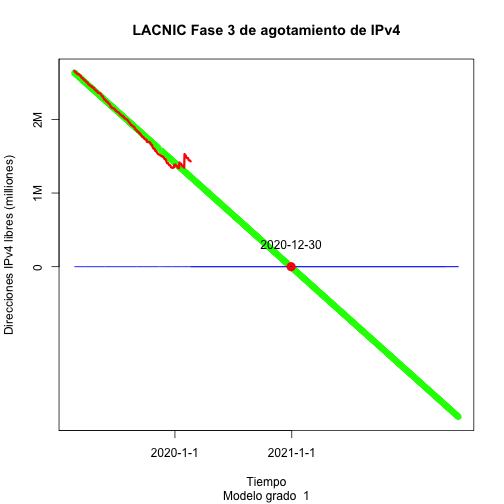
\includegraphics{LACNIC_IPv4_F3_Report_v3_files/figure-beamer/unnamed-chunk-2-1.pdf}

\end{frame}

\begin{frame}{Modelo de grado 2}
\protect\hypertarget{modelo-de-grado-2}{}

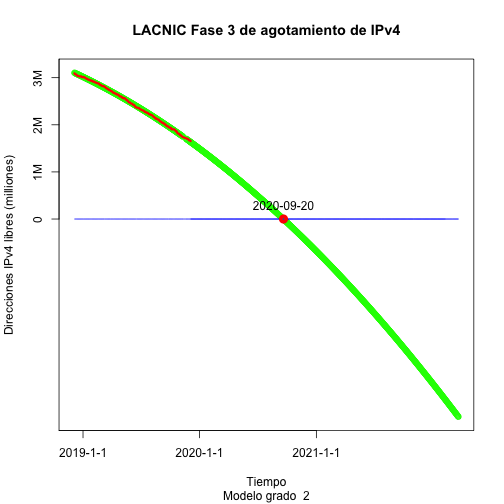
\includegraphics{LACNIC_IPv4_F3_Report_v3_files/figure-beamer/unnamed-chunk-3-1.pdf}

\end{frame}

\begin{frame}{Modelo de grado 3}
\protect\hypertarget{modelo-de-grado-3}{}

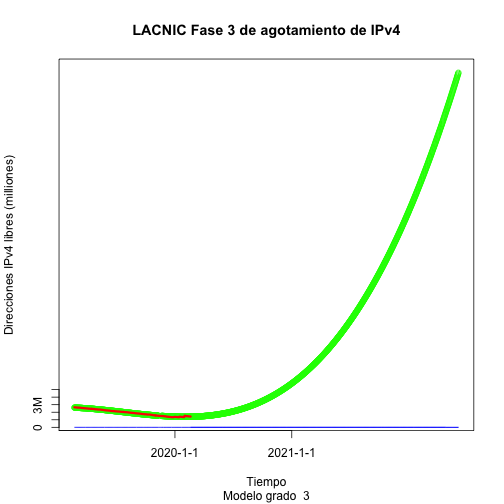
\includegraphics{LACNIC_IPv4_F3_Report_v3_files/figure-beamer/unnamed-chunk-4-1.pdf}

\end{frame}

\begin{frame}[fragile]{Fechas de agotamiento}
\protect\hypertarget{fechas-de-agotamiento}{}

La predicción de fechas de agotamiento de acuerdo a los diferentes
modelos es:

\begin{itemize}
\tightlist
\item
  Grado 1:
\end{itemize}

\begin{verbatim}
## [1] "2020-12-07"
\end{verbatim}

\begin{itemize}
\tightlist
\item
  Grado 2:
\end{itemize}

\begin{verbatim}
## [1] "2020-08-17"
\end{verbatim}

\begin{itemize}
\tightlist
\item
  Grado 3:
\end{itemize}

\begin{verbatim}
## [1] NA
\end{verbatim}

\end{frame}

\end{document}
